\section{Boundary Conditions (BC)}
\subsection{Interface Conditions}

\begin{minipage}[lt]{8cm}
	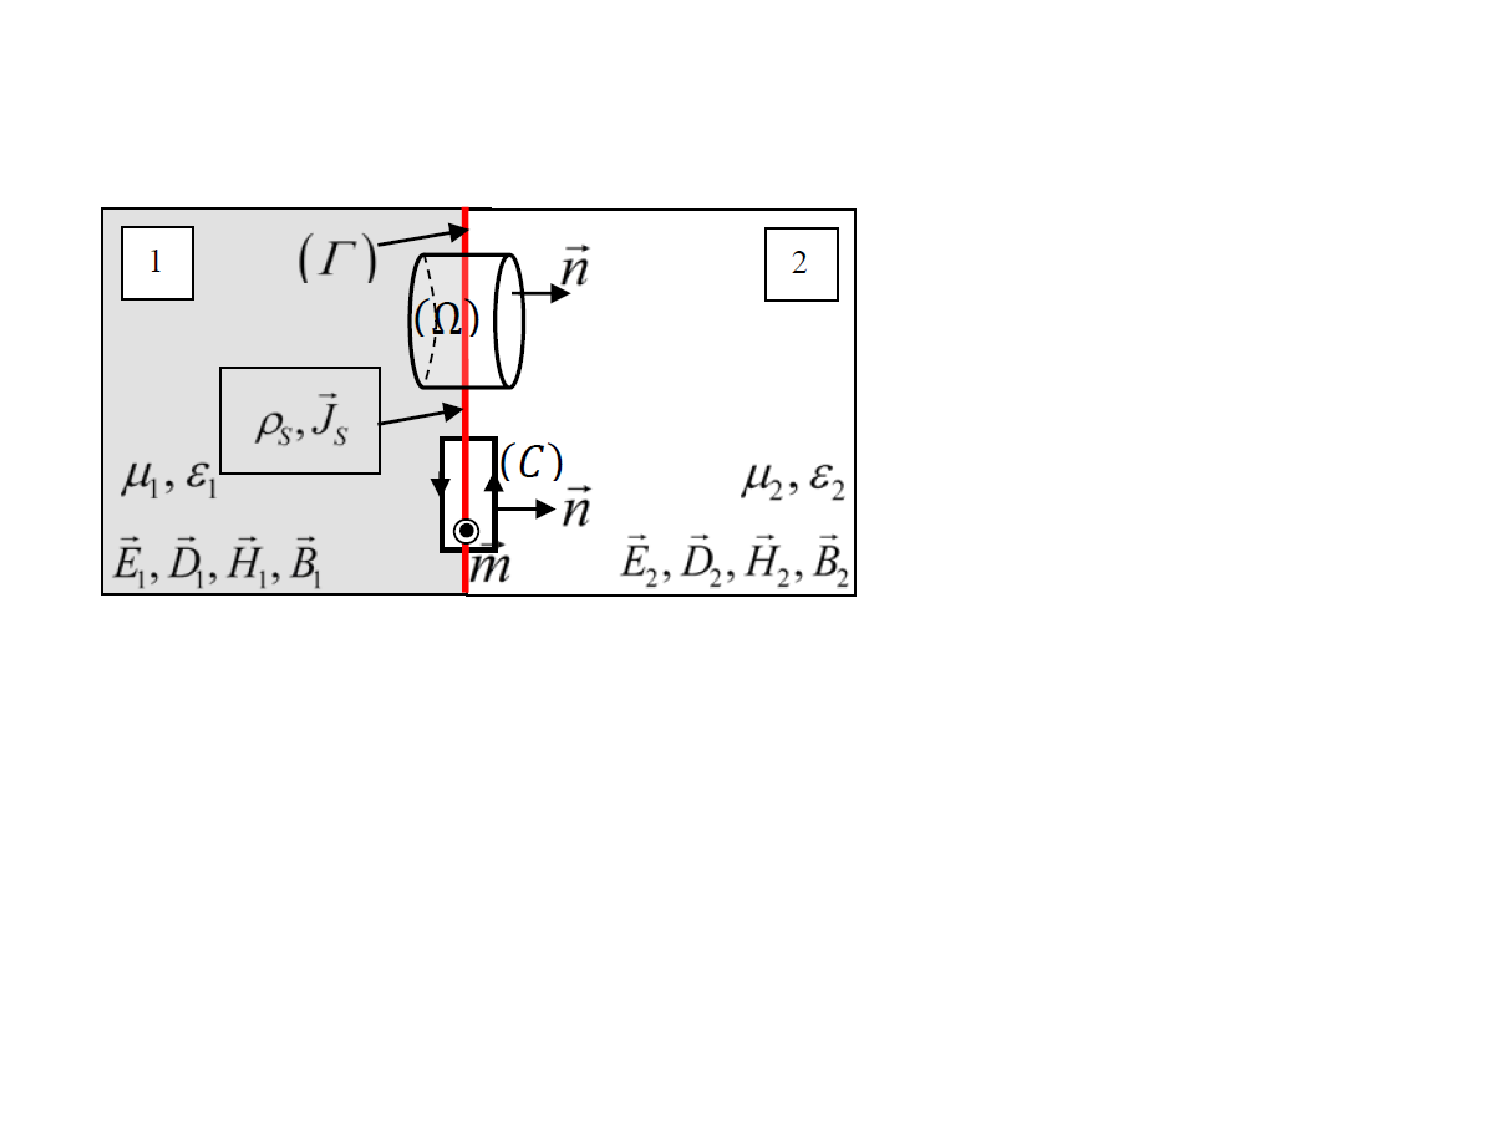
\includegraphics[width=.8\textwidth]{./images/InterfaceConditions.pdf}
\end{minipage}
\begin{minipage}[rt]{11cm}
	\begin{tabular}{l}
		$\left(\vec{D}_1 - \vec{D}_2\right) \cdot \vec{n} = \rho_S$ \\
		$\left(\vec{B}_1 - \vec{B}_2\right) \cdot \vec{n} = 0$\\
		$\left(\vec{H}_2 - \vec{H}_1\right) \times \vec{n} =\vec{J}_S$ \\
		$\left(\vec{E}_2 - \vec{E}_1\right) \times \vec{n} = 0$\\
	\end{tabular}
\end{minipage}
The above interface conditions show the field behavior over the border between two different materials. \newline
The normal flux density continuity conditions can be derived by integrating Equations (1) and (2) over the cylinder $\Omega$ depicted above. \newline
The tangential field continuity conditions can be proven by integrating Equations (3) and (4) along the contour $C$ shown above.